\chapter{Choix et justifications}

\section{Émetteurs infrarouges}

Concernant les émetteurs infrarouges, des LEDs pourront être utilisées. En effet, la distance écran/utilisateur ne sera pas très grande, et de simple LEDs seront suffisantes pour éclairer la pupille de l'utilisateur. Nous pourrons par exemple utiliser l’Émetteur infrarouge (IR) Kingbright L-934SF4BT (880 nm 50 ° 3 mm) ou alors l’Émetteur infrarouge (IR) Harvatek HT-159IRAJ 940 nm 20 ° 1206 CMS coûtant respectivement 0.90€ et 0.35€ pièce. Le choix se fera en fonction des connectiques nécessaires (la première LED offre une sortie radiale avec des connecteurs UY2, alors que la seconde se présente sous forme de puce).

\section{Caméras}

Si de nombreux types de caméras sont possible, nous avons retenu la webcam. En effet, la résolution des webcams HD actuelles est largement suffisante pour une détection de pupille. De plus, elles sont facilement utilisables via des ordinateurs, c'est-à-dire simple d'installation et il est aisé de récupérer les flux vidéos. Leur connexion USB facilite elle aussi leur utilisation. Nous pouvons également noter que les webcams sont relativement peu coûteuses.


\subsection{Caméras «grand-angle»}

Pour le suivi du visage, la Webcam LOGILINK USB avec LED a été retenue. Elle est compatible avec Windows, Mac et Ubuntu et ne posera donc pas de problème de compatibilité. De plus elle possède un système lui permettant de pivoter sur 360° permettant ainsi le meilleur suivi du visage possible. Cependant, d'autres webcams présentent ces avantages et le détail qui nous a décidé dans ce choix est la présence de LEDs (voir figure \ref{fig:LEDCam}). En effet, trois LEDs sont présentes de chaque coté de l'objectif et pourraient éventuellement être remplacées par des émetteurs infrarouges.

\begin{figure}[H]
  \centering
  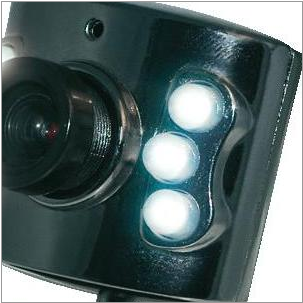
\includegraphics[scale=0.5]{LEDCam}
  \caption{Présence de LEDs sur la webcam}
  \label{fig:LEDCam}
\end{figure}

Le placement des LEDs sur la webcam pourrait nous éviter de devoir mettre en place un système pour pouvoir brancher ces LEDs.


\subsection{Caméras «petit-angle»}

Ensuite, concernant la caméra petit-angle, la Webcam Trust Widescrenn Full HD 1080p (voir figure \ref{fig:CamPetitAngle}) a été choisie. D'abord parce que le tacking des pupilles demande une grande résolution et que cette webcam est adapté à la résolution Full HD 1080p (1920x1080), mais aussi parce qu'elle intègre une éclairage LED permettant, comme précédemment, de placer nos émetteurs infrarouges.

\begin{figure}[H]
  \centering
  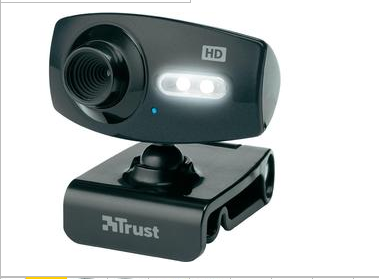
\includegraphics[scale=0.5]{CamPetitAngle}
  \caption{Webcam Trust Widescrenn Full HD 1080p}
  \label{fig:CamPetitAngle}
\end{figure}Émetteur infrarouge




\chapter{Résultats et analyses}

analyse des tests et des performances
analyse des échecs, des décalages et des retards
Que reste-t-il à faire ? Comment ?


